\documentclass[11pt]{scrartcl}
\usepackage{graphicx}
\usepackage{float}
\usepackage[utf8]{inputenc}
\usepackage[spanish]{babel}

\title{\textbf{Java: historia de una libertad cuestionada}}
\subtitle{Legal Aspects - MSWL URJC}
\author{Ricardo García Fernández}
\date{\today}

\begin{document}

\maketitle

\newpage

\tableofcontents

\newpage

\section{Introducción}

La vida de Java como tecnología está llena de caminos en el filo de la navaja entre los mundos de lo privativo, lo libre y la libertad. Este es un resumen a groso modo de la historia de la tecnología Java desde sus inicios hasta la fecha de hoy \date{\today}.\\
La presentación de Java como una tecnología de desarrollo libre desde distintos puntos de vista mediante el estudio de las licencias que lo han acompañado, los encuentros y desencuentros con la comunidad de desarrolladores y la absorción de Sun por la empresa Oracle.

\section{El inicio de Java}

Java comenzó como una tecnología de desarrollo para ser usado en un set-top-box\footnote{http://es.wikipedia.org/wiki/Set-top\_box} en 1991 donde inicialmente se bautizó como \emph{Oak}, pasando más adelante a llamarse \emph{Green} hasta que finalmente llegó el nombre que perduró y perdura; Java.
Todos estos cambios de nombre fueron debidos a que colisionaban con distintas marcas ya registradas en aquella época, desde el principio se ven atisbos de las tormentas que luego llegarían.\\
El equipo de desarrolladores estaba encabezado por \emph{James Gosling}\footnote{http://en.wikipedia.org/wiki/James\_Gosling}, un desarrollador canadiense iniciador de esta historia. La presentación de Java al mundo data de su primera versión publicada en 1995, que fue una \emph{alpha y beta}, hasta la primera versión estable en 1996 la \emph{1.0} en la que se incluía la máquina virtual JVM.\\
Java es un lenguaje que destaca por su máxima "write once, run anywhere" (WORA), es decir se puede desarrollar una aplicación y al compilarse ésta ya es funcional en cualquier tipo de entorno, no es necesario volverla a compilar en la plataforma de destino. Esta afirmación encierra por debajo un detalle importante el cual nos presenta una máquina virtual encargada de hacer que el software funcione en cada plataforma la JVM\footnote{http://www.java.com/es/download/manual.jsp?locale=es} - \emph{Java Virtual Machine} que no es libre, aquí se presenta el primer escollo para la libertad, para poder ejecutarlo en cualquier entorno ha de usado bajo la máquina virtual propietaria con la implementación de Sun.

\section{JVM: la libertad de...}

Una cosa está clara, Java es un lenguaje de programación libre, si nos acotamos al lenguaje en si. La instalación en nuestro sistema operativo de la versión JDK (Java Development Kit) nos da la posibilidad de utilizar el lenguaje para crear lo que necesitemos mediante su sintaxis haciéndolo funcionar a través de su máquina virtual (JVM).\\
Como se puede ver, hay dos fases en el desarrollo de un software mediante Java:
\begin{enumerate}
    \item Desarrollar el Software (incluyo la compilación considerando la compilación como Software en si para el tratamiento en este texto).
    \item Ejecutar el Software indistintamente del entorno.
\end{enumerate}

En el segundo punto nos detenemos ya que es ahí donde Java restringe la libertad y obliga a pasar por su máquina virtual mediante su implementación.

\section{Conociendo a los actores}

Pudiendo tener un software libre implementado en Java pero teniendo que ejecutarse a través de un software privativo por lo que no es completa la libertad de uso al programa.\\
¿ Es posible crear una máquina virtual propia que interprete el lenguaje Java y de esta forma crear un ciclo del software completamente libre ? Si pero no puede ser Java ya que tenías que ir Sun pagar por la licencia de esa herramienta pasando los tests TCK (technology compatibility kit) para que pudiera ser 'java compliant' o dicho de otra manera, reconocida como máquina virtual para ejecutar aplicaciones Java.
Esta parte es por donde Sun/Oracle han cerrado puertas a los desarrolladores a través de la historia no permitiendo la evolución, al ser una implementación privada, alrededor de Java que es una de las mayores comunidades de desarollo y de los lenguajes más demandados.

En este caso donde chocan las libertades podemos contemplar a cinco actores en la historia de Java; Free Software Foundation, Apache Software Foundation, Sun (más tarde absorvida por Oracle) y Google.

\subsection{Free Software Foundation}

Empezaremos por la FSF que por medio de Richard Stallman mediante la redacción de artículos y especificaciones en licencias relacionadas con Java y su JVM.

\subsubsection{Java trap}

El primer artículo 'La trampa de Java'\footnote{http://www.gnu.org/philosophy/java-trap.es.html} escrito en el año 2004 describe la posición de la FSF recomendando el no uso de la JVM por los desarrolladores Java:

\begin{quotation}
    \emph{Si usted escribe un programa en Java sobre la plataforma Java de Sun, está expuesto a usar funcionalidades exclusivas de Sun sin ni siquiera darse cuenta. Para cuando se dé cuenta, quizás las haya estado usando durante meses, y rehacer el trabajo le tomaría más meses. Podría decir «volver a empezar es demasiado trabajo». Entonces su programa habrá caído en la trampa del Java; será inusable en el mundo Libre.}
\end{quotation}

Este extracto del texto es el más significativo con respecto a Java y su uso de la JVM en donde nos emplaza al uso de máquinas virtuales Java libres que van haciéndose hueco en el mercado.
La FSF puso en marcha el proyecto GCJ - \emph{The GNU Compiler for the Java} utilizando los ejemplos de éxito del compilador libre de C (GCC\footnote{http://www.gnu.org/software/gcc/releases.html}) que ofreció una alternativa libre para desarrollar bajo el lenguaje C en entornos libres cuando no existían opciones.

\subsubsection{GNU Classpath}

A la par, también se creó el proyecto \emph{GNU Classpath}\footnote{http://www.gnu.org/software/classpath/} que aglutina las librerías Java principales para incluirlas en máquinas virtuales de Java y desarrollar bajo esta estructura de una forma completamente libre.
El proyecto GNU Classpath está publicado bajo GPLv2 (y posteriores) en donde se incluye una cláusula asociada a la licencia:

\begin{quotation}
    \emph{Linking this library statically or dynamically with other modules is making a combined work based on this library. Thus, the terms and conditions of the GNU General Public License cover the whole combination.\\
    As a special exception, the copyright holders of this library give you permission to link this library with independent modules to produce an executable, regardless of the license terms of these independent modules, and to copy and distribute the resulting executable under terms of your choice, provided that you also meet, for each linked independent module, the terms and conditions of the license of that module. An independent module is a module which is not derived from or based on this library. If you modify this library, you may extend this exception to your version of the library, but you are not obligated to do so. If you do not wish to do so, delete this exception statement from your version.}
\end{quotation}

As such, it can be used to run, create and distribute a large class of applications and applets. When GNU Classpath is used unmodified as the core class library for a virtual machine, compiler for the java languge, or for a program written in the java programming language it does not affect the licensing for.

En donde destacamos que si se utiliza como módulo de un software sin modificación alguna la licencia GPL no afecta al licenciamiento de el software creado, es decir no es un programa derivado y actúa como biblioteca para que de esta forma no influya si se utiliza en la creación de una máquina virtual y esto implique que todo el código deba ser licenciado bajo la misma licencia, GPLv2 y posterior.

\subsubsection{The Curious Incident of Sun in the Night-Time}

En 2006 la empresa Sun empezó a plantearse la publicación de Java como código GPL, mientras la FSF seguía crítica después del anuncio de la propia empresa de publicar pero bajo un acuerdo de no divulgación (NDA inglés) para que los binarios de la JVM pudiesen ser publicados bajo una distribución GNU/Linux, es decir incluir por defecto su intérprete para la expansión de su uso. Caso el cual la FSF no tuvo en consideración debido a que no seguía los criterios de Software Libre ya que seguía aparecer el código fuente:

\begin{quotation}
    \emph{Si examinamos con atención el anuncio de Sun, veremos que representa exactamente estos hechos. No menciona que la plataforma de Java sea software libre, ni siquiera de código abierto. Únicamente predice que la plataforma estará «extensamente disponible» en las «principales plataformas de código abierto». Disponible, es decir, como software privativo, en términos que nos niegan libertad.}
\end{quotation}

Por lo que la noticia, llamada no noticia por la FSF en el artículo 'El curioso incidente de Sun a durante la noche'\footnote{http://www.gnu.org/philosophy/sun-in-night-time.html} sirvió para continuar adviertiendo del mal uso de Software Libre alrededor de la tecnología Java y continuó a la expectativa del próximo movimiento de la compañía con respecto a su política de libertad, más que nunca observada.

\subsection{Apache Software Foundation}

¿ Donde se encuentra la Fundación Apache en este instante ? La Fundación Apache (ASF) es una de las grandes precursoras Java y las libertades del Software por lo que han recorrido un largo camino juntos.\\
Podemos ver que hay un total de 162 proyectos realizados en Java en la página web de 'ASF projects'\footnote{http://projects.apache.org/indexes/language.html\#Java} en comparación con C de los que Apache mantiene 18. A simple vista se puede apreciar la colaboración entre Java y ASF. Dentro de los cuales destaca el proyecto \emph{Apache Harmony}, una implementación de Java propia. La ASF también estaba preocupada por la implementación libre de Java ya que la mayoría de sus proyectos dependen de esta tecnología.

\subsubsection{Conflicto con Java SE 7}

La ASF ha sido un miembro muy activo dentro de la evolución de Java mediante su puesto en el comité ejecutivo de la Java Community Process en el que ha sido nombrado Miembro del Año 4 veces a lo largo de los 10 años que ocupó el puesto. Puesto que dejó atrás debido a sus discrepancias\footnote{http://blogs.apache.org/foundation/date/20101209} con respecto al proceso de licenciamiento sobre \emph{Java SE7}:

\begin{quotation}
    \emph{Oracle provided the EC with a Java SE 7 specification request and license that are self-contradictory, severely restrict distribution of independent implementations of the spec, and most importantly, prohibit the distribution of independent open source implementations of the spec.}
\end{quotation}
    
Oracle como dueño de Sun aboga por imponer sus normas por encima de la comunidad con más de 10 años de experiencia en el modelo evolutivo de Java (1998 a 2010), por lo que ASF promueve la no aceptación por parte del Comité Ejecutivo (EC) de la \emph{JCP} de la versión 7 pero se encuentra con un proceso viciado por intereses empresariales que le afectan directamente a ellos mismos como fundación y por tanto a todos los desarrolladores de Java.

Apache llevaba desde 2007 indagando y exponiendo la liberación de los test bajo una licencia libre para poder certificar, esgrimiendo delante de Sun (primero) hasta Oracle que la imposición de normativas en la JCP estaba violando las normas de la misma JCP como describe la 'open letter' de Apache a Sun en 2007\footnote{http://www.apache.org/jcp/sunopenletter.html} donde pone como ejemplos las mismas normas:

\begin{quotation}
  \emph{1) a specification lead cannot "impose any contractual condition
     or covenant that would limit or restrict the right of any
     licensee to create or distribute such Independent
     Implementations" (section 5.C.III)}

  \emph{2) a specification lead must license all necessary IP
     royalty-free to any compatible implementation of a
     specification (section 5.B)}
\end{quotation}

Oracle no acepta que el proyecto Harmony como válido para pasar los test de la \emph{TCK license} por lo que priva a los desarrollodores de Java de una implementación oficial libre en la que puedan respaldar sus proyectos violando las libertades añadiendo restricciones privativas a las licencias TCK para ser incompatibles con las licencias libres\footnote{http://blogs.apache.org/foundation/entry/statement\_by\_the\_asf\_board1}:

\begin{quotation}
    \emph{Through the JSPA, the agreement under which both Oracle and the ASF participate in the JCP, the ASF has been entitled to a license for the test kit for Java SE (the "TCK") that will allow the ASF to test and distribute a release of the Apache Harmony project under the Apache License. Oracle is violating their contractual obligation as set forth under the rules of the JCP by only offering a TCK license that imposes additional terms and conditions that are not compatible with open source or Free software licenses. The ASF believes that any specification lead that doesn't follow the JCP rules should not be able to participate as a member in good standing, and we have exercised our votes on JSRs -- our only real power on the JCP -- accordingly.  We have voted against Sun starting and continuing JSRs, and have made it clear that we would vote against the JSR for Java SE 7 for these reasons.}
\end{quotation}

Por lo que la ASF acaba diciendo sobre la JCP \emph{"JCP specifications are nothing more than proprietary documentation."} y retirándose del comité debido a la falta de democratización e incursión de Oracle en las propias decisiones de la comunidad como empresa propietaria mediante el licenciamiento privativa que coarta la libertad de obtener una \emph{VM licenciada por TCK libre}.

El proyecto Harmony acaba abandonado por la ASF en el mes de Noviembre del año 2011. Google heredó el proyecto para crear su propia implementación de Java. 

\subsection{Sun}

Para conocer un poco más a la empresa Sun hemos de verla como empresa delante de una estrategia comercial flirteando con ambos bandos.

Sun como hemos expuesto en los inicios de Java creó la implementación para uso privado haciéndolo expansible paultinamente y ganando adeptos exponencialmente debido a su versatilidad, fluidez y facilidad que otorgaba Java al desarrollo. Pudiendo un progama compilado en Java ser ejecutado en cualquier máquina que posea la JVM, la suya.La implementación de Java creada por ello ha de ser la única oficial además de su propia máquina virtual.
La licencia con la que se distribuía inicialmente Java es la \emph{Java Research License}\footnote{http://www.java.net/jrl.csp} en la que explícitamente se refiere al uso en el investigación alrededor del mundo académico para usos no comerciales. Esta licencia por lo tanto no es libre ya que restringe la libertad a un único ámbito siendo incompatible con GPL además de no estar aprovada por la OSI ni por la FSF.

Java Community Process\footnote{http://www.jcp.org/en/home/index} \emph{JCP} es una organización que fue creada en 1998 desde la versión J2SE 1.4 por Sun para que estandarizar a través de la comunidad los desarrollos técnicos de Java y la evolución del lenguaje. Es una comunidad abierta a los colaboradores en donde se proponen y someten a votación los estándares mediante los \emph{Java Specification Requests JSRs} o las evoluciones del mismo lenguaje mediante las \emph{Java Language Specification JLS}. Estas mejoras pueden ser promovidos por cualquier persona de la comuniada para así mejorar Java a través de la gente que más lo usa y por lo tanto más está interesada en que mejore.

En el año 2006 Sun veía como el proyecto se posicionaba de nuevo arriba con un pequeño descenso respecto a la demanda y uso.

\begin{figure}[H]
  \centering
  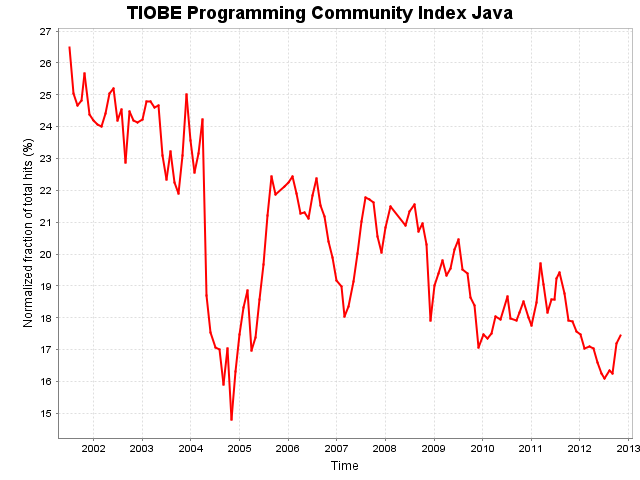
\includegraphics[width=0.8\textwidth]{images/history_Java}
  \caption{TIOBE Java}
  \label{fig:tiobejava}
\end{figure}

El impulso de la comunidad a través de la JCP y las presiones bien intencionadas por parte de la FSF y ASF de liberar el código fuente bajo una licencia libre dieron sus frutos.\\
Por lo que podemos ver Java se encontraba flanqueada por varios bandos y de capa caída por lo que tomó la decisión de licenciar bajo una licencia de Software Libre. Se decidió finalmente por la GPLv2 en vez de \emph{Common Development and Distribution License (CDDL)}\footnote{http://directory.fsf.org/wiki/License:CDDLv1.0} que es incompatible a su vez con la GPLv2 por ser de copyleft fuerte. La FSF no recomienda su uso debido a la incompatibilidad con su licencia y el apartado que le dedica lamentándose que en el texto de la licencia se utilice la definición de propiedad intelectual.

Sun liberó el \emph{OpenSDK bajo GPLv2}, de esta forma accedía a las peticiones de la JCP y la comunidad, con un pero. La liberación de Java bajo \emph{GPLv2 con la cláusula classpath}\footnote{http://openjdk.java.net/legal/gplv2+ce.html}. De la que podemos extraer que si alguien modifica o evoluciona el OpenJDK debe de estar disponible para todo el mundo como así dicta la Licencia GPL pero acogiéndose a la cláusula del classpath puede cerrar su código mientras lo certifique a través de Sun por las TCK por lo que de esta forma gana un dinero y hace que las mejoras no sean públicas debido a que ella misma es la empresa que crea la implementación y la que certifica las implementaciones.

Este es un uso de la licencia \emph{GPLv2 con cláusula classpath} pero desde otro punto de vista, la FSF, la cláusula fue creada para que la licencia GPLv2 no se aplicase como vírica afectando a cualquier software que tuviese contacto con el licenciado y el proyecto tuviese una aceptación mayor para impulsar el proyecto Classpath.

\subsection{Sun becomes Oracle}

Oracle se aprovecha de la fragilidad que tenía Sun en el año 2009 acumulando pérdidas y vence en la pugna que mantenía con IBM por la compra de Sun.

Entra en juego un nuevo actor del mundo privativo directamente dentro de una empresa que siempre había estado en el otro lado. Este es un hecho importante dentro de la evolución de Java hacia adelante ya que la empresa se torna oscura y no tan comprensiva con respecto a la comunidad de Software Libre. Podemos aunque seamos repetitivos fijarnos en la gráfica de nuevo para ver el momento exacto del tiempo estableciendo un paralelismo con el declive en pérdidas por parte de Sun y la adquisición de la compañía por parte de Oracle por la incertidumbre que esto significaba dentro del desarrollo de Software Libre.

Oracle empezó entrando de lleno en la JCP e intentando asociarse para su beneficio, lícitamente claro está ya que es la empresa creadora del proyecto y ha tutelado la evolución del mismo desde sus inicios.

El hito más impactante de Oracle dentro de la JCP es el que se le relaciona con la negativa de facilitar la certificación de las implementaciones de Java como la Apache Harmony a partir de los estándares libres definidos en la JCP. Esta certificación posibilitaba que Apache con su proyecto publicara la implementación bajo los estándares mediante la licenciación Apache Version 2.0 imponiendo que al licenciarse a través de las TCKs sea privado y por lo tanto no se pudiese liberar incompatibilizándolo con las licencias de Software Libre mediante la imposición de normas restrictivas dentro de la comunidad abierta que era la JCP.

Tomó como apoyo a IBM y consiguió que no se facilitara una implementación robusta y fiable como la de Apache Harmony bajo una Licencia Libre. Es decir siguió apoyando lo que en un principio impulsó Sun, defiendo sus derechos como empresa para que la certificación implicase una privatización del código imposibilitando la publicación como Software Libre.

El abandono de Apache fue un antes y un después con el que nos enlaza la incursión del siguiente actor.

\subsection{Google}

Google dio el salto a las tecnologías móviles con Android. ¿ Que es el lenguaje AndroidSDK ? sencillamente AndroidSDK es una implementación de Java propia a partir del proyecto Harmony de Apache licenciado, esta es la parte importante, por una licencia de Software Libre \emph{Apache version 2.0}\footnote{http://source.android.com/source/licenses.html}. Implementó una máquina virtual propia llamada Dalvik\footnote{http://code.google.com/p/dalvik/} desde cero para utilizar con su implementación.

En este par de párrafos a groso modo introducimos a Google en el centro de la tormenta de las licencias con lo que respecta a Java y por consiguiente a la empresa Oracle su propietaria.

Google implementó su propio Java conocido como \emph{AndroidSDK}\footnote{http://developer.android.com/sdk/index.html} e hizo que se expandiese de una manera muy rápida estando en boca de todos, le dio vida y subsistencia, al publicarlo bajo una Licencia de Software Libre.

Oracle por su parte se vio delante de un nuevo frente que no dudó en abrir en 2010 mediante una demanda por infracción de copyright y violación de patentes (aquí encontramos una explicación más detallada\footnote{http://www.groklaw.net/article.php?story=20100815110101756}) para salvaguardar su producto y evitar que otros actores ganaser poder de decisión sobre la evolución de otra implementación distinta a la suya además del uso de una nueva VM ajena a ellos.

Podemos dividir la demanda de Oracle sobre Google en dos partes diferenciadas:
\begin{enumerate}
    \item Infracción del copyright al utilizar Java. Un ataque directo por el uso de Java en los terminales móviles sin contar con JavaME.
    \item Uso de patentes en la máquina virtual Dalvik. Las patentes definidas en la demanda pertenecen al grupo de patentes básicas para la creación de una máquina virtual por lo que podría demandar a cualquier persona/empresa/colectivo que construyese una VM.
\end{enumerate}

La demanda se tildó de paranoica debido a que nadie veía ningún fundamento ya que la implementación no tuvo que pasar por los test TCK y la VM era una implementación nueva específica para la misma implementación. La licencia lo permitía, creó una competencia virtual acabando, como se ha visto con el tiempo, con la especificación JavaME de un plumazo. Las nuevas plataformas móviles han adoptado con agrado la plataforma Android (que proviene de Linux) utilizando su lenguaje (es Java pero no se llama Java) debido a la licencia por la que optó Google, una licencia libre.

La resolución de la demanda falló en favor de Google\footnote{http://www.fayerwayer.com/2012/05/juez-google-no-tendra-que-pagarle-nada-a-oracle-no-infringio-copyright/} por lo que la libertad del desarrollo de software quedó garantizada. El Software Libre en base a sus Licencias protegió al desarrollador, en este caso a una empresa, al ejercer su libertad mediante los medios estipulados, las licencias, la buena elección de una licencia.

\subsection{James Gosling}

No nos acordábamos que todo nació de su mente y del equipo de personas que trabajabaron con él; Arthur Van Hoff\footnote{http://www.linkedin.com/in/aavanhoff}, y Andy Bechtolsheim\footnote{http://en.wikipedia.org/wiki/Andy\_Bechtolsheim}.

Jamas Gosling es el creador pero no el propietario de Java, el propietario de Java es la empresa Sun. Gosling como creador puede tener influencia en su desarrollo y aportar ideas alrededor de la estrategia comercial de Sun(después Oracle) pero no es el licenciador de la tecnología y la última y válida palabra es la que ejerce Sun.

Abandonó Oracle en el en 2010\footnote{http://nighthacks.com/roller/jag/entry/time\_to\_move\_on}, el año más convulso para la compañía. Después de su salida la compañía, la misma se torno más opaca, empezando con la demanda de Oracle a Google y la guerra interna dentro de la JCP con la ASF que hizo que ASF dejara el comité ejecutivo. Gosling nos deja una referencia en su blog personal de lo que supuso para el y a ojos de la comunidad la demanda de Oracle sobre Google por el uso de Java y el incumplimiento de determinadas patentes "The shit finally hits the fan"\footnote{http://nighthacks.com/roller/jag/entry/the\_shit\_finally\_hits\_the}, la mierda ha llegado finalmente al ventilador. Esta frase crea un paralalelismo perfecto describiendo el momento exacto de Oracle, parece que da espadazos sin sentido a ver con lo que topa y tiende a ser el camino del principio la pérdida de muchas miradas de la gente con respecto a Java y esto último es muy personal para Gosling.

\section{Post\-valoración}

Volvemos a echar la vista al gráfico de la evolución de Java durante esta época y podemos darnos cuenta que entrando en el año 2010 la popularidad de Java sufrió un varapalo importante del que parecía haberse recuperado un año más tarde en 2011 después de haber sorteado el \emph{annus horribilis}\footnote{http://en.wikipedia.org/wiki/Annus\_horribilis}. Más adelante a partir de la mitad de 2011 se aprecia claramente en la gráfica la caída en picado. Dejó de bajar a mediados de 2012, de nuevo a mínimos en comparación consigo misma, coincidiendo el punto de reflotación con la resolución de la senticia sobre la demanda fallando a favor de Google. A partir de este instante, Java vuelve a subir como la espuma.

Podremos decir que la sentencia a favor de Google salvaguarda el desarrollo abierto de una implementación de Java, por parte en este caso de una empresa, y la no violación de ninguna patente por parte de la sentencia. Por lo tanto la comunidad respira y Oracle sigue al acecho de Google.

Una derrota victoriosa de Oracle.

\section{Implementaciones Alternativas}

Como hemos comentado se han creado alternativas a la JVM oficial de Java e implementaciones bajo Licencias de Software Libre, aquí hay un pequeño resumen de las más conocidas como referencias:
\begin{itemize}
    \item Dalvik - Google Virtual Machine\footnote{http://code.google.com/p/dalvik/} para ejecutar aplicaciones Android.
    \item AndroidSDK - La implementación de Java creada por Google\footnote{http://developer.android.com/sdk/index.html} a partir del proyecto Apache Harmony\footnote{http://harmony.apache.org/} retirado de la Apache Software Foundation.
    \item Hotspot - OpenJDK Virtual Machine\footnote{http://openjdk.java.net/groups/hotspot/}.
    \item Kaffe - Kaffe is a clean room implementation of the Java virtual machine, plus the associated class libraries needed to provide a Java runtime environment\footnote{http://www.kaffe.org/}.
    \item OpenJDK - The place to collaborate on an open-source implementation of the Java Platform, Standard Edition, and related projects\footnote{http://openjdk.java.net/}.
    \item GCJ - The GNU Compiler for the Java\footnote{http://gcc.gnu.org/java/}.
\end{itemize}

\begin{thebibliography}{9}

    \bibitem{javahistory}
        Java, historia y presente. Sus actores. La ida de Apache de JCP,\\
        Martín Alejandro Casco,\\
        http://elsoftwarelibre.wordpress.com/2010/12/10/java-historia-y-presente-sus-actores-la-ida-de-apache-de-jcp/
    \bibitem{javamica}
        ¿El principio del fin de Java?,\\
        Micael Gallego Carrillo,\\
        http://sidelab.wordpress.com/2010/08/16/el-principio-del-fin-de-java/
\end{thebibliography}

\end{document}
